\section{Cross-Language Equivalence Checking with SMACK}

In this work, we explore equivalence checking of functions written originally in
the C programming language that are translated into Rust programming language
versions of the function, which should be equivalent.
%
Our main focus is on verifying correct translation of a native Rust language
math library compared to the source C language version of the math functions.
%
Additionally, because floating-point math can be unintuitive, a math library
might have subtle errors related to unintentional replacements in the
translation, for example, by applying familiar algebraic simplifications that
may not be appropriate to apply to floating point calculations.

Cross-language equivalence checking in SMACK is done by exploiting its ability
to handle programs written in multiple programming languages.
%
Because SMACK works mainly on the LLVM and Boogie levels, rather than working
directly on source-level languages, SMACK needs to have some source level main
program which ties together functions to be verified.

There are some identities that are true, for example $2.0*x = x+x$ and $3.0*x =
x+x+x$ for 32-bit floating-point numbers.
%
Using the default floating-point rounding-mode, round to nearest ties to even,
it is even true that $4.0*x = x+x+x+x$ and $5.0*x=x+x+x+x+x$.
%
Given this, we may convince ourselves that $n*x=x+x+\cdots+x$ where $n$ is an
integer and the sum on the right is adding $x$ to itself $n$ times.
%
In the following example, we will show how to set up SMACK to verify that $5.0*x
= x+x+x+x+x$ for 32-bit floating-point numbers.
%
In the Rust program in~\cref{fig:rustcfivex}, we have the function
\texttt{rust\_five\_x} on \cref{line:rustfivex}, which computes $5.0*x$.
%
Similarly, the C program in~\cref{fig:rustcfivex} computes $x+x+x+x+x$ in the
function \texttt{c\_five\_x} on~\cref{line:cfivex}.
%
We now have two functions we want to verify their equality.

Because of SMACK is a software verifier, we need to create a verification
harness which ties the two programs together, in this case the function
\texttt{main} on~\cref{line:fivexharness} of the Rust program in~\cref{fig:rustcfivex}.
%
\footnote{We chose to write the verification harness in Rust due to a preference
for its syntax. It is possible to do this the other way where the \texttt{main}
function calls a Rust function from a C program instead.}
%
The first step of the harness function is to create a common input, \texttt{x}
(line~\ref{line:xcreate}), for both functions we wish to check for equivalence.
%
This input is a \textit{nondeterministic} value, created through SMACK's
\texttt{nondet} family of functions.
%
This input variable is then constrained~(\cref{line:xconstrain}) to not be
NaN because this will produce NaN results, which are always unequal.
%
Then, the two functions we wish to check for equality are called with the
common input \texttt{x} as their argument, and their return values captured
(lines~\ref{line:fivexccall} and~\ref{line:fivexrustcall}).
%
Finally, the call to \texttt{verifier\_assert}~(\cref{line:fivexassert}) directs
the verifier to check if the two return values are equal.

When we run SMACK on these files, it compiles the two programs to LLVM bytecode,
links them into one program, then translates it to Boogie for verification.
%
On this example, SMACK reports no errors, meaning the two functions are
equivalent, for inputs that are not NaN.

%There are two functions we are testing for equivalence: the Rust function \texttt{rust\_compute} (line~\ref{line:rustcomp} of listing~\ref{lst:examplerust}), and the C language version of this program, \texttt{c\_compute} (line~\ref{line:ccomp} of listing~\ref{lst:examplec}).
%
%Boogie then turns this program into an SMT query then an SMT solver then tries to show the formula is unsatisfiable or find a counter example.

Now we can use SMACK to check if this pattern holds for $6.0*x = x+x+x+x+x+x$.
%
We setup the two programs (shown in \cref{fig:crustsixx}) similar to
the prior example, but updating the calculations.
%
When we use SMACK on these programs, it reports an error and shows a
counter-example.

% \begin{figure}[tb]
% \noindent\begin{minipage}{.49\textwidth}
% \begin{lstlisting}[frame=tb, language=Rust, label={lst:rustsixx}, caption={Rust code.}, style=boxed, escapechar=`, basicstyle=\small]
% fn rust_six_x(x: f32) -> f32 {`\label{line:rustsixx}`
%   return 6.0*x;
% }
% \end{lstlisting}
% \end{minipage}
% %
% \begin{minipage}{.49\textwidth}
% \begin{lstlisting}[frame=tb, language=C, label={lst:csixx}, caption={C Code.}, style=boxed, escapechar=`, basicstyle=\small]
% float c_six_x(float x) {`\label{line:csixx}`
%   return x+x+x+x+x+x;
% }
% \end{lstlisting}
% \end{minipage}
% \caption{An example of a program written in Rust and a program written in C which may seem to be equivalent.}
% \end{figure}

In this example, SMACK produces the counter-example $x=9.223373136366404e+18$.
%
We can verify that $6.0*x=5.534024101722168e+19$ while
$x+x+x+x+x+x=5.534023661917517e+19$.
%
We can get SMACK to produce a counter-example that is easier to work with by
restricting the range of possible values for $x$ by adding, for example, the
constraint \texttt{verifier\_assume!(0.5 < x \&\& x < 1.0)}.
%
With this constraint, we may get $x=0.5950928330421448$ as a counter example
with $6.0*x=3.570557117462158$ and $x+x+x+x+x+x=3.570556879043579$.
%
If we sum the numbers, we can see that the final addition rounds in the opposite
direction of the multiplication.
%
Note that specific counter-examples generated by SMACK can be influenced by
solver version, program structure, variable names, etc, and these may not be the
exact values given by SMACK.
% Unconstrained nondeterministic values in SMACK. Emphasize symbolic execution, Boogie and SMT.
% Reads as if it's a kind of testing.
% Set up of the harness.
% Why this works.
% Assert outputs are equivalent.
% 
% 2.2 Background on SMACK
% 2.3 Scalability tricks
% Cross product of paths
%
%In this example the harness logically executes the C-language program before the Rust language program.
%
%This means that in the query issued to the solver, the return value from the C-language program is known symbolically prior to the symbolic execution of the Rust program.
%
%We note this to emphasize that the two programs are not treated by SMACK as if they are treated as if they are running in parallel.
%
%The harness runs both programs and saves the results from both.
%
%Finally, the both results are tested for equality.
%
%If the two values are equivalent, then SMACK has shown that the two programs are equivalent.
%
%Otherwise, SMACK has shown the two programs may not be equal for all possible inputs.
%\zvon{I think ideally you should have initially two functions that are not equivalent.
%Then you explain the setup. Then you say, ok, when we run SMACK on this, it says
%that they are not equivalent. It also gives us a counterexample with inputs that
%lead to them not being equivalent.
%Then you fix it and show the fixed listing. Then you say we run SMACK again
%and now it shows that they are equivalent.}

% Breaking inputs for this example: x = 0.9353114366531372
% c_res = 0.7652881741523743, rust_res = 0.7652881145477295.
% These results are different because floating point math is not associative.
% In these two calculations, there are two rounding steps and the result may
% differ if the calculation is x*(x*(x*x))) or (x*x)*(x*x).

\subsection{Scalability}

In this work, we encountered numerous examples where verification tasks did not
finish.
%
While this is a well known issue in software verification, we developed some
techniques to help with verification performance on this class of programs.

\subsection{Over-Approximation of Theories}
The simplest approach is to first run SMACK without modeling floating-point or
bit-vector operations.
%
If SMACK reports no errors, then the functions are equivalent since SMACK was
able to show that both functions perform identical operations on their inputs.
%
If SMACK does report an error, we first try enabling the floating point model
without enabling the bit-vector theory since it is expensive to transfer between
these two theories.

\subsection{Restrict Operations To Not Produce NaN}
This may not always make verification go through, so additional approaches are
needed.
%
One approach is to transform the program so that floating-point
arithmetic-operations are constrained to not produce NaN values.
%
We use a Boogie program pass to transform the program so that the results of
floating-point addition, subtraction, multiplication and division are
constrained to not be NaN values.
%
This helps verification because if the two programs are equivalent, then the
solver won't be able to find a counter-example.
%
NaN values are not equal to any floating-point values -- including NaN -- so the
solver is essentially attempting to prove NaN values are not possible.
%
If the program is prevented from considering NaN values, then the solver can
prove that the non-NaN version of the functions are equivalent.
%
When doing this transformation, once the programs are shown to be equivalent
absent NaN values, the program can then be shown to not produce NaN values.

\subsection{Guided Equivalence Checking}
Finally, we introduce a mechanism where we can try to guide the solver to focus
on specific paths in the program to show that corresponding variables in the two
programs are equivalent.
%
We do this using new verifier functionality to store values from one
program, then use another function to check that another value in the other
program are equal.
%
We demonstrate this in \cref{fig:storeequiv}.
%
Naively, when examining these programs as a pair, the paths through the
C-language function are independent of the paths through the Rust-language
function.
%
There are 16 potential paths through the combined programs.
%
We use \texttt{verifier\_equiv\_store(value)} to store the value of a
variable on this path to be loaded later.
%
In the Rust-language program, we use \texttt{verifier\_equiv\_check(value)} to verify the stored value from the C-language program is the same as the
value in the Rust-language program.
%
This does significantly reduce solving time for many programs, partially because
it guides the solver toward learning that the paths through the two programs
are the same, e.g., in this example, the four paths in the C-language program
are the same as the four paths through the Rust-language program, reducing the
number of potential paths to four from sixteen.

In addition to helping the SMT solver match equivalent expressions between the two programs, this also helps the solver constrain the possible values on checked values.
%
Because the check is done according to FP-equality, if the two expressions are shown to be equivalent, they are also shown to not produce NaN values.
%
This enables a solver to reduce the expressions, which makes equivalence checking dependent expressions easier.

\subsection{Equivalence Checking Extensions}

% \begin{figure}[tb]
%   \centering
%   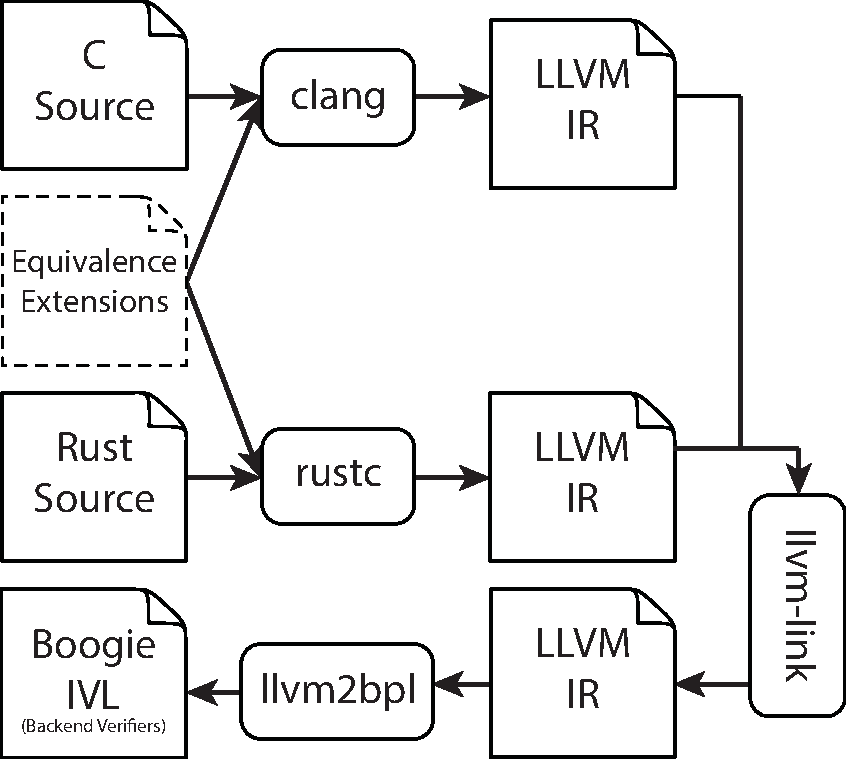
\includegraphics[width=0.92\textwidth]{chap4/fig/SmackEquiv.pdf}
%   \caption{Equivalence checking extensions within SMACK.}
%   \label{fig:toolflow}
% \end{figure}

We added equivalence checking extensions to SMACK, so they are available generally from the tool.
%
These extensions are represented in the ``equivalence extensions'' part of~\cref{fig:toolflow}.
%
The \texttt{verifier\_equiv\_store} functions are implemented in Boogie as shown in~\cref{line:equiv-assume}, where \texttt{\$foeq} is SMACK's floating-point equivalence function corresponding to the SMT-LIB floating-point equality function, \texttt{fp.eq}.
%
We use a global counter \texttt{equiv\_store\\\_counter} to track each value stored in this way.
%
This value is incremented with each use, so as to maintain unique identifiers for retrieving values from \texttt{verifier\_equiv\_store}.
%
This uses the theory of uninterpreted functions to allow the value to effectively be retrieved later.

The \texttt{verifier\_equiv\_check} functions are implemented in Boogie as shown in~\cref{line:equiv-assert} of~\cref{lst:equivstore}.
%
This adds an assertion that the value we are checking is equal to the value stored previously.
%
This also uses a distinct counter to create unique identifiers for the values stored, and increases this value similar to the \texttt{verifier\_equiv\_store} function.
%
The \texttt{verifier\_equiv\_assume} function is implemented similarly.

The use of automatically generated identifiers adds the requirement that uses of \\ \texttt{verifier\_equiv\_check} must occur in the same order and number as uses of \texttt{verifier\\\_equiv\_store}.
%
This is to allow for values inside loops to be checked without associating multiple values to stored values with the same identifier, potentially making the program trivially correct.
%
It is because of this that we introduce the \texttt{verifier\_equiv\_assume} function to allow the user to verify the program, one check at a time.

% \begin{figure}[tb]
% \begin{lstlisting}[label={lst:equivstore}, caption={verifier\_equiv\_store code}, style=boxed, escapechar=`]
% function verifier_store(x: int) returns (float);

% var store_counter: int = 0;
% var load_counter: int = 0;

% procedure verifier_equiv_store(x: float) {`\label{line:equiv-assume}`
%   assume $foeq(x, verifier_store(store_counter));
%   store_counter := store_counter + 1;
% }

% procedure verifier_equiv_check(x: float) {`\label{line:equiv-assert}`
%   assert $foeq(x, verifier_store(load_counter));
%   load_counter := load_counter + 1;
% }
% \end{lstlisting}
% \end{figure}

% \begin{figure}[tb]
% \noindent\begin{minipage}{.47\textwidth}
% \begin{lstlisting}[language=C, label={lst:cstore}, caption={C equivalence}, style=boxed, escapechar=`]
% float c_computation(float x) {
%   float y = 2.0 * x;
%   if(x < -1.0) {
%     y += 1.0;
%     verifier_equiv_store(y);
%   }
%   else if(x <= 0.0) {
%     y -= 1.0;
%     verifier_equiv_store(y);
%   }
%   else if(x <= 1.0) {
%     y *= 2.0;
%     verifier_equiv_store(y);
%   }
%   else {
%     y /= 2.0;
%     verifier_equiv_store(y);
%   }
%   return y;
% }
% \end{lstlisting}
% \end{minipage}
% %
% \begin{minipage}{.52\textwidth}
% \begin{lstlisting}[language=Rust, label={lst:rustequiv}, caption={Rust equivalence}, style=boxed, escapechar=`]
% fn rust_computation(x: f32) -> f32 {
%   let mut y = 2.0 * x;
%   if x < -1.0 {
%     y += 1.0;
%     verifier_equiv_check(y);
%   }
%   else if x <= 0.0 {
%     y -= 1.0;
%     verifier_equiv_check(y);
%   }
%   else if x <= 1.0 {
%     y *= 2.0;
%     verifier_equiv_check(y);
%   }
%   else {
%     y /= 2.0;
%     verifier_equiv_check(y);
%   }
%   return y;
% }
% \end{lstlisting}
% \end{minipage}
% \end{figure}

\subsection{Experiments Using SMT Equivalence}
We investigated the impacts non-equivalence of NaN values has on showing equivalence of expressions in this work.
%
We conducted an experiment where we replaced \\ SMACK's floating-point equivalence functions (\texttt{\$foeq}) as being defined in terms of the SMT equivalence relation, i.e., by defining the \texttt{\$foeq} functions to be the built-in \texttt{=} in Boogie.
%
We used this alternate definition on some of the longer running benchmarks and found they made the assertion checks faster, sometimes by a factor of 10.
%
This suggests that the proof obligation of the solver to show that the expressions are free from NaN values is responsible for some of the scalibility issues we encountered.
%
It should be noted that while there may be some merit in treating NaN values as equivalent only when comparing equality of returned values, this transformation is not sound.
%
For example, the expression \texttt{x != x} should be true when \texttt{x} is NaN.
%
This means that control flow may be affected by treating NaN values as equivalent.